\documentclass{article}

\usepackage{graphicx}
\usepackage{tikz}
\usepackage{tikzsymbols}
\usetikzlibrary{calc,patterns,shapes.geometric}
\pagestyle{empty}
\usepackage[margin=0pt]{geometry}
\geometry{papersize={14in,12in}}

\def\centerarc[#1](#2)(#3:#4:#5){\draw[#1] ($(#2)+({#5*cos(#3)},{#5*sin(#3)})$) arc (#3:#4:#5);}

\begin{document}
	\begin{figure}
		\centering
		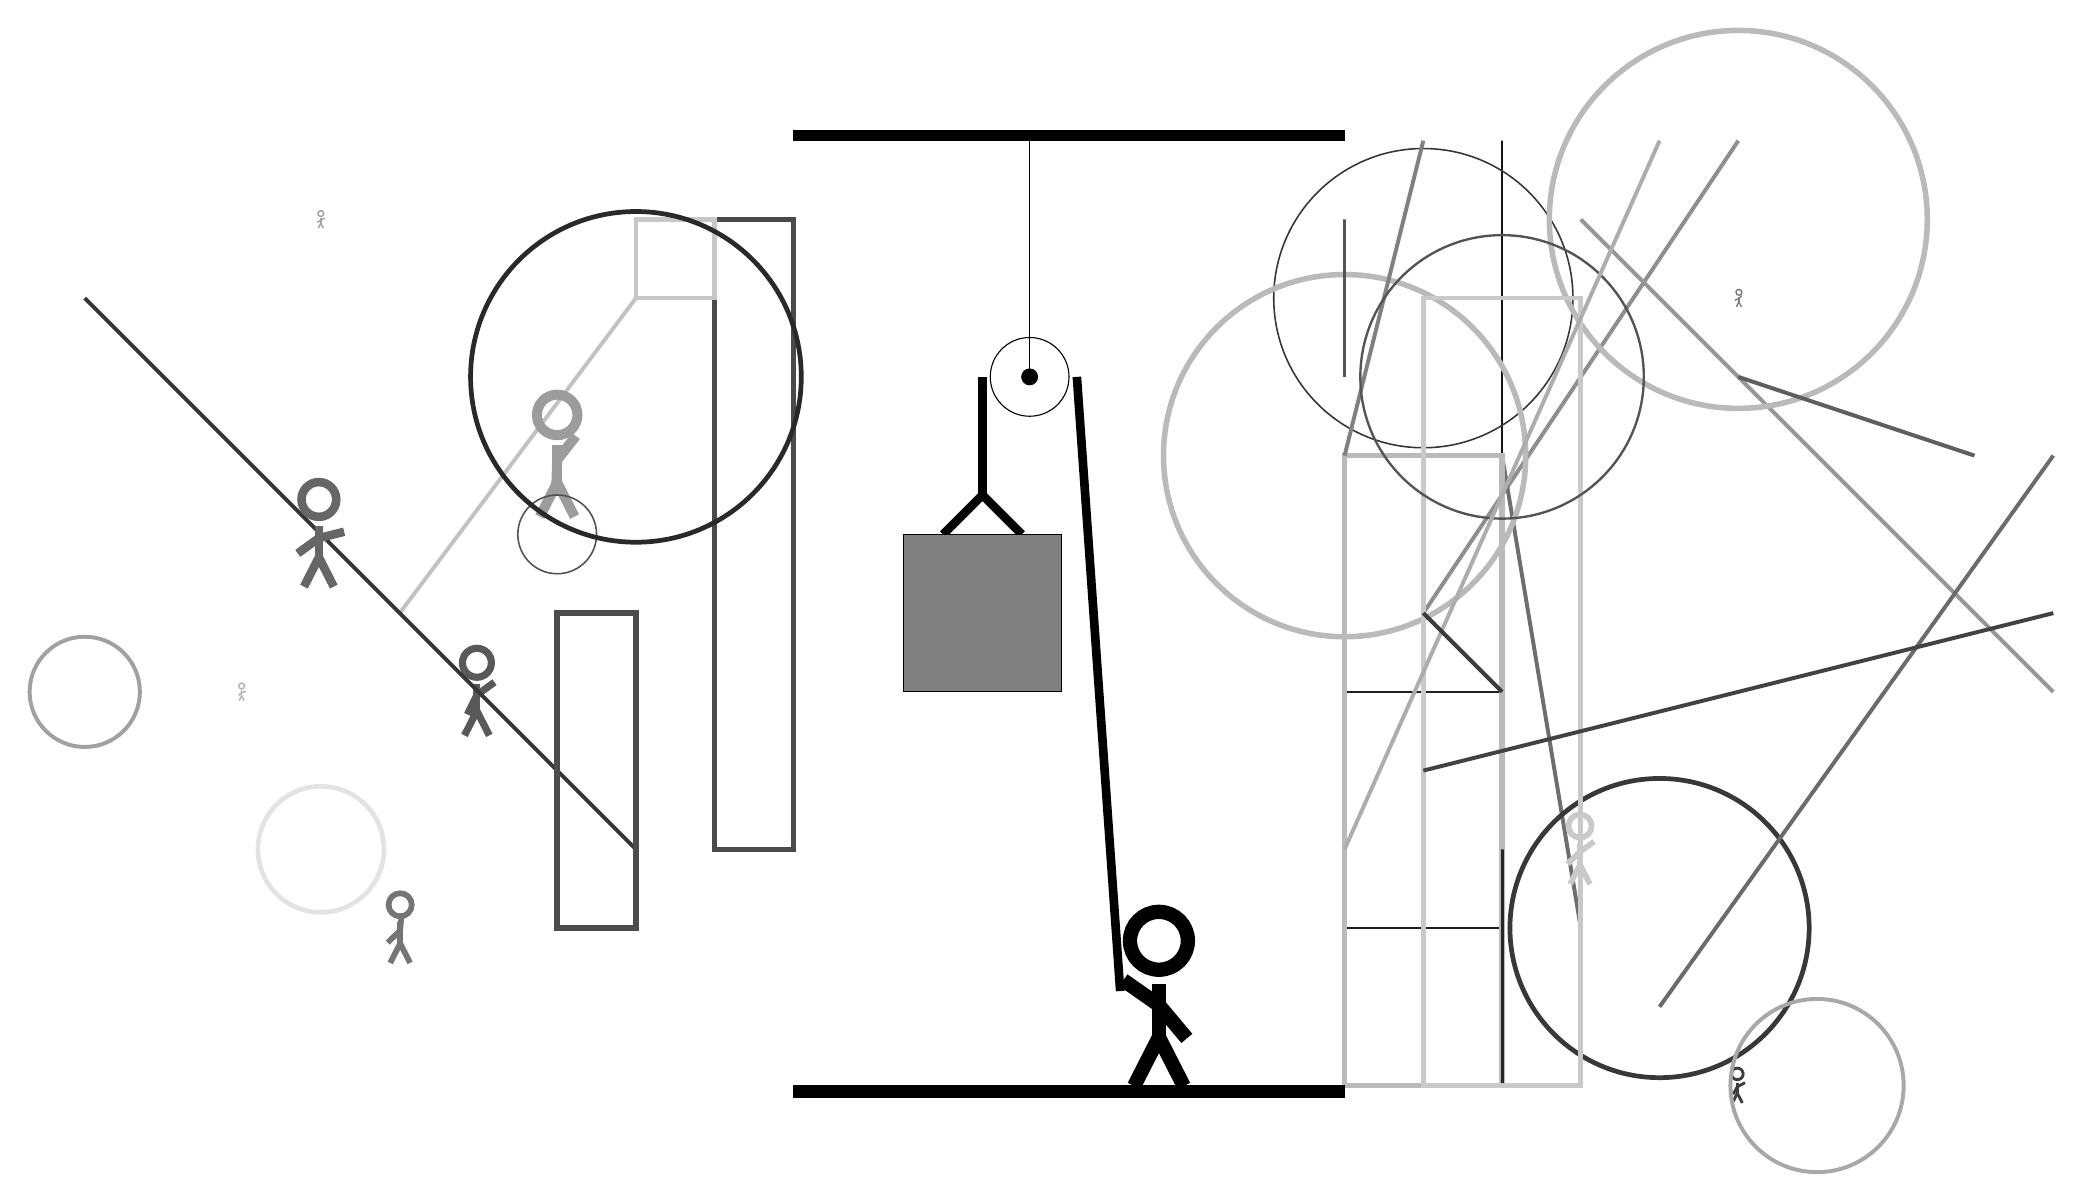
\begin{tikzpicture}
			%%%%% START %%%%%
			
			\draw[fill=black] (-2, 9) rectangle (5, 9.125);
			
			\draw (1, 6) circle (0.5);
			\draw[fill=black] (1, 6) circle (0.1);
			\draw (1, 9) -- (1, 6);
			
			\draw[line width=1.1mm] (-0.1, 4.0) -- (0.4, 4.5) -- (0.9, 4.0);
			\draw[fill=black!50] (-0.6, 4.0) rectangle (1.4, 2.0);
			
			\node[line width=0.6mm, color=black!51] at (10, 7) {\Strichmaxerl[1][19][49]};
			
			\draw [line width=0.7mm, color=black!52](10, 1) circle (0.0);
			\draw[line width=0.2mm, color=black!92] (7, 9) rectangle (7, 2);
			\draw[line width=0.5mm, color=black!44](6, 3) -- (10, 9);
			
			\node[line width=0.5mm, color=black!37] at (-8, 8) {\Strichmaxerl[1][35][25]};
			\draw[line width=0.3mm, color=black!88] (7, 2) rectangle (5, -1);
			
			\draw[line width=0.5mm, color=black!78] (6, 2) rectangle (6, 1);
			
			\draw [line width=0.2mm, color=black!79](6, 7) circle (1.9);
			\draw[line width=0.5mm, color=black!57](8, -1) -- (7, 5);
			\draw [line width=0.7mm, color=black!27](5, 5) circle (2.3);
			\draw [line width=0.6mm, color=black!11](-8, 0) circle (0.8);
			
			\node[line width=0.7mm, color=black!65] at (-6, 2) {\Strichmaxerl[5][64][36]};
			\draw[line width=0.5mm, color=black!24](-4, 7) -- (-7, 3);
			
			\draw [line width=0.6mm, color=black!78](9, -1) circle (1.9);
			\draw[line width=0.7mm, color=black!27] (5, 5) rectangle (7, -3);
			\draw[line width=0.5mm, color=black!41](8, 8) -- (14, 2);
			\node[line width=0.6mm, color=black!39] at (-5, 5) {\Strichmaxerl[7][88][52]};
			\draw[line width=0.5mm, color=black!50](5, 5) -- (6, 9);
			\node[line width=0.2mm, color=black!76] at (10, -3) {\Strichmaxerl[2][60][28]};
			\node[line width=0.3mm, color=black!30] at (-9, 2) {\Strichmaxerl[1][45][11]};
			\draw[line width=0.4mm, color=black!85] (7, -3) rectangle (7, 0);
			\draw [line width=0.5mm, color=black!34](11, -3) circle (1.1);
			\draw [line width=0.7mm, color=black!27](10, 8) circle (2.4);
			\draw[line width=0.5mm, color=black!58](9, -2) -- (14, 5);
			\draw[line width=0.5mm, color=black!79](-4, 0) -- (-11, 7);
			
			\draw[line width=0.6mm, color=black!71] (-2, 0) rectangle (-3, 8);
			\draw[line width=0.6mm, color=black!21] (6, 7) rectangle (8, -3);
			\draw[line width=0.6mm, color=black!22] (-3, 8) rectangle (-4, 7);
			
			\draw [line width=0.3mm, color=black!67](7, 6) circle (1.8);
			
			\node[line width=0.7mm, color=black!54] at (-7, -1) {\Strichmaxerl[4][44][85]};
			\draw[line width=0.5mm, color=black!74](6, 1) -- (14, 3);
			\draw [line width=0.2mm, color=black!68](-5, 4) circle (0.5);
			\draw [line width=0.5mm, color=black!37](-11, 2) circle (0.7);
			\draw[line width=0.5mm, color=black!32](5, 0) -- (9, 9);
			\node[line width=0.2mm, color=black!21] at (8, 0) {\Strichmaxerl[4][44][36]};
			\draw[line width=0.5mm, color=black!63](10, 6) -- (13, 5);
			
			\draw [line width=0.6mm, color=black!84](-4, 6) circle (2.1);
			
			\draw[line width=0.5mm, color=black!77](6, 3) -- (7, 2);
			\draw[line width=0.7mm, color=black!70] (-4, 3) rectangle (-5, -1);
			\node[line width=0.4mm, color=black!60] at (-8, 4) {\Strichmaxerl[6][36][14]};
			\draw[line width=0.3mm, color=black!67] (5, 8) rectangle (5, 6);
			
			
			\draw[line width=1.1mm] (0.4, 6) -- (0.4, 4.5);
			\centerarc[line width=1.1mm](1, 6)(0:180:0.6);
			\draw[line width=1.1mm](1.6, 6) -- (2.15, -1.8);
			
			\node at (2.6, -1.9) {\Strichmaxerl[10][-35][-50]};
			
			\draw[fill=black] (-2, -3) rectangle (5, -3.15);
			
			%%%%% END %%%%%
		\end{tikzpicture}
	\end{figure}	
\end{document}